\documentclass[10pt]{article}
\usepackage{icmlko}

\icmlmeta{IP 파운데이션 월드모델}{275}{열 번째 도메인}{학습 문턱 40 대 15 는 판이 못 정한다 --- 그 문턱이 가르는 것은 판이 제일 못 보는 도메인 하나다}

\begin{document}

\twocolumn[
\icmlheader

\begin{abstract}
서 있던 갈래 하나를 닫았다 --- \textbf{학습 문턱 40 을 15 로 내릴까.}
저장된 이벤트는 07-30 에 t15 판 \textbf{0.4498} · t40 판 \textbf{0.4391}
을 적었다. $+$0.0107 이면 노트 245의 미결정 폭 0.010 을 겨우 넘는다.
\textbf{짝지어 재니 $+$0.0011 (t${=}$0.42)} 이었고 F21 은 $+$0.0002 였다.
\texttt{spread} 의 진짜 총량은 \textbf{0.0000 · 진짜 0개}. \textbf{저장된
차가 열 배 부풀어 있었다} --- 노트 274가 오늘 두 번 잡은 병의 세 번째다.
그리고 문턱이 실제로 무엇을 가르는지 셌다: 배포 규약 학습행이
세계애니 2,648 부터 아이돌 54 까지인데 \textbf{팝업만 16 이다.} 두 문턱
사이에 있는 도메인이 정확히 하나고, 그것이 이 프로젝트의 출발점이다.
문턱을 내리면 학습 도메인이 9 $\to$ 10 이 되고 \textbf{팝업이 $+$0.0317}
(짝SE 0.0270 · $t{=}1.17$)을 얻는다. 나머지 아홉은 $|t|{<}0.6$ 이다.
노트 274가 어제 세운 법칙이 이 수를 미리 말한다 --- 팝업의 몫이 2.3\% 라
$0.0317 \times 0.023 = +0.0007$ 이고 판에서 잰 값은 $+$0.0011 이다.
\textbf{판은 이 문턱을 정할 수 없다.} 그래서 정하는 자리를 옮겼다:
\textbf{판이 무차별할 때는 배포가 정한다.} $|\Delta|{=}0.0011$ 은 미결정
폭의 9분의 1 이고, 배포 쪽에서는 출발점이 $+$0.0317 을 공짜로 받는다.
\textbf{t15 로 간다} --- 판이 그렇게 말해서가 아니라 판이 아무 말도 못
해서다.
\end{abstract}
]

\section{닫으려고 연 갈래}

서 있는 갈래 목록의 첫 줄이 오래 이랬다.

\begin{quote}\small
학습 문턱 40 $\to$ 15 를 전 판에서 재확정(팝업만 영향, 나머지 아홉은 이미
40 이상).
\end{quote}

근거는 저장된 이벤트였다.

\begin{center}\small
\begin{tabular}{lll}
\hline
시각 & 이벤트 & 판 \\
\hline
07-30 16:29 & 학습 문턱 40 & \\
07-30 16:45 & 도전 최고 \texttt{@trendcalwiki} & $+$0.4391 \\
07-30 16:45 & 학습 문턱 15 & \\
07-30 16:56 & \texttt{@trendcalwiki·t15} 가드 통과 & $+$0.4498 \\
\hline
\end{tabular}
\end{center}

$+$0.0107 이다. 노트 245가 정한 미결정 폭 0.010 을 아슬아슬하게 넘어서,
``확정만 하면 되는 것''처럼 보였다.

\textbf{두 실행이다.} 노트 274가 오늘 아침에 적은 규약이 정확히 이걸
금지한다 --- 저장된 점수는 실행을 가로질러 빼지 않는다.

\section{$+$0.0011}

\begin{figure*}[t]
\centering
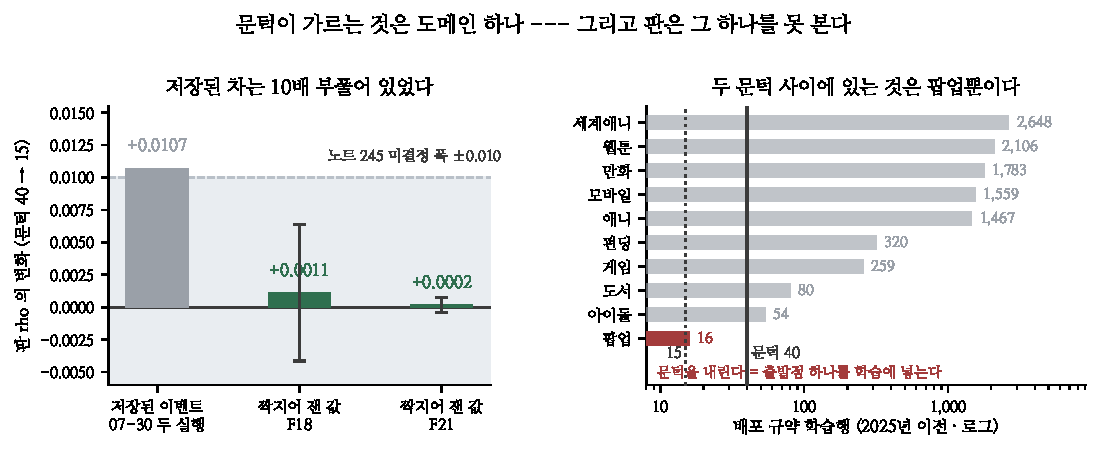
\includegraphics[width=\textwidth]{figs/thresh.pdf}
\caption{왼쪽 --- 문턱 40 $\to$ 15 의 판 변화. 회색 띠가 노트 245의 미결정
폭 $\pm$0.010 이다. 저장된 차만 밖에 있고 짝지어 잰 둘은 안에 있다.
오른쪽 --- 배포 규약이 실제로 쓰는 학습행. 두 문턱 사이에 팝업 하나뿐이다.}
\end{figure*}

같은 씨앗(0 · 1 · 2)으로 문턱만 바꿔 짝지어 쟀다.

\begin{center}\small
\begin{tabular}{lrrr}
\hline
& 문턱 40 & 문턱 15 & 짝 차 \\
\hline
학습 도메인 & 9 & \textbf{10} & \\
F18 판 & 0.4845 & 0.4857 & $+$0.0011 ($t{=}0.42$) \\
F21 판 & 0.4542 & 0.4544 & $+$0.0002 ($t{=}0.68$) \\
\hline
\textbf{팝업} & 0.361 & \textbf{0.393} & \textbf{$+$0.0317} ($t{=}1.17$) \\
도서 & 0.369 & 0.377 & $+$0.0084 ($t{=}0.50$) \\
펀딩 & 0.267 & 0.258 & $-$0.0094 ($t{=}{-}0.57$) \\
아이돌 & 0.137 & 0.129 & \\
웹툰 & 0.453 & 0.451 & \\
애니 & 0.505 & 0.502 & \\
\hline
\end{tabular}
\end{center}

\texttt{rank.spread} 의 \emph{진짜 총량}은 \textbf{0.0000 · 진짜 0개}다.
\textbf{저장된 $+$0.0107 은 열 배 부풀어 있었다.}

오늘만 세 번째다. 노트 274에서 팝업의 $-$0.067(실제 $+$0.0071)과 웹툰
마스킹의 $-$0.069(진짜 0개)를 잡았고, 이번이 셋째다. \textbf{병이 하나고
자리가 셋이다.}

\section{문턱이 정확히 무엇을 가르나}

배포 규약이 쓰는 학습행(2025년 이전)을 도메인마다 셌다.

\begin{center}\small
\begin{tabular}{lr@{\qquad}lr}
\hline
도메인 & 학습행 & 도메인 & 학습행 \\
\hline
세계애니 & 2,648 & 펀딩 & 320 \\
웹툰 & 2,106 & 게임 & 259 \\
만화 & 1,783 & 도서 & 80 \\
모바일 & 1,559 & 아이돌 & 54 \\
애니 & 1,467 & \textbf{팝업} & \textbf{16} \\
\hline
\end{tabular}
\end{center}

\textbf{두 문턱 사이에 있는 것은 팝업 하나다.} 40 에서 둘째로 작은
아이돌(54)까지 여유가 14 행이고, 팝업은 15 와 40 사이에 혼자 앉아 있다.
그러니 이 문턱 논쟁은 처음부터 \textbf{``출발점의 16행을 학습에 넣을까''}
하나였다.

넣으면 팝업이 $+$0.0317 을 얻는다. 이것은 노트 254가 아홉 도메인에 물었던
질문(제 학습이 제게 이로운가)의 \textbf{열 번째 답}이다. 노트 254는
도서만 제 학습이 해롭다고 했는데, 그때 팝업은 문턱 밖이라 물을 수조차
없었다. \textbf{물어 보니 팝업도 나머지 여덟 편이다.}

\section{그런데 판이 못 정한다}

노트 274가 어제 세운 법칙을 여기 그대로 대 본다. 도메인 하나의 이득이
판에 실리는 값은 그 도메인의 몫을 곱한 값이다.

\begin{center}\small
\begin{tabular}{lr}
\hline
팝업이 얻은 값 & $+$0.0317 \\
팝업의 유보 몫 & 2.3\% \\
판에 실릴 값(예상) & $+$0.0007 \\
\hline
판에서 잰 값 & \textbf{$+$0.0011} \\
미결정 폭(노트 245) & 0.010 \\
\hline
\end{tabular}
\end{center}

\textbf{미결정 폭의 9분의 1 이다.} 노트 274의 표가 팝업에 대해 적은
수(판이 쓰려면 도메인 안에서 $\Delta\rho{=}0.435$)를 생각하면 놀랄 일이
아니다 --- $+$0.0317 은 그 14분의 1 이다.

\textbf{판은 이 문턱에 대해 아무 말도 못 한다.} 그리고 노트 274가
보인 대로 \emph{앞으로도} 못 한다. 문턱이 가르는 유일한 도메인이 하필
판이 제일 못 보는 도메인이기 때문이다.

\section{그래서 정하는 자리를 옮긴다}

순위가 못 정하면 안 정하는 것이 지금까지의 기본값이었다. 그건 t40 을
유지한다는 뜻이고, \textbf{유지도 결정이다} --- 출발점을 학습에서 빼
두는 결정.

여기서 노트 254의 구분을 실제로 쓴다.

\begin{quote}\small
판정 단위와 배포 단위는 다르다. 도구를 팝업에 쓰는 사람에게는 판의
가중이 아무 의미가 없다.
\end{quote}

\textbf{규칙 하나를 세운다.} 어떤 변경이 (1) 판에서 미결정 폭 안이고
(2) 어느 도메인에서도 $|t|{>}2$ 로 나빠지지 않으면, \textbf{배포 쪽 이득이
정한다.} 이번 변경은 둘 다 만족한다 --- 판 $+$0.0011, 제일 나쁜 도메인이
펀딩 $-$0.0094 ($t{=}{-}0.57$).

\textbf{t15 로 간다.} 판이 그렇게 말해서가 아니라 \textbf{판이 아무 말도
못 해서}다. 이건 순위 규칙을 무르는 게 아니다 --- 순위 규칙은 미결정
구간에서 자기가 못 정한다고 이미 말하고 있고(노트 245), 그 구간에서
무엇으로 정할지는 여태 안 적혀 있었다.

\paragraph{조심할 것} 이 규칙은 \textbf{미결정 폭 안에서만} 산다. 폭
밖이면 판이 정한다. 그리고 (2)를 뺀 채로 쓰면 작은 도메인을 올리려고
큰 도메인을 조금씩 깎는 변경이 줄줄이 통과한다 --- 노트 247 · 248이 잰
상쇄가 정확히 그 모양이었다.

\paragraph{남은 것}
\begin{center}\small
\begin{tabular}{ll}
\hline
갈래 & 왜 \\
\hline
t15 로 재승격 & 챔피언을 문턱 15 에서 다시 뽑아야 \\
팝업 전용 축 & 이제 배포 기준이 있으니 값이 생겼다 \\
저장에 시각·해시 & 오늘 세 번 같은 병에 걸렸다 \\
펀딩 $-$0.0094 & 두 노트째 음수. 아직 $t{=}{-}0.6$ \\
\hline
\end{tabular}
\end{center}

\paragraph{규약} \textbf{판이 미결정이라고 말할 때 그것은 ``유지''가
아니라 ``판 밖에서 정하라''는 뜻이다.} 그리고 \textbf{문턱 · 가중치 같은
설정을 바꿀 때는 그것이 실제로 무엇을 가르는지 먼저 센다} --- 이번에
문턱 40 대 15 는 판 전체의 문제처럼 보였지만 실은 도메인 하나, 행 16개의
문제였다.

\end{document}
